\chapter[Feasibility Design Study: Password Reuse Manager]{Feasibility Design Study: \\Password Reuse Manager}\label{chap:pwrm}

\section{Background and Context}
Password managers (PWMs) are one of the common coping strategies for an ever growing number of accounts. 
% übergang zu dem noch ausformulieren. 
Zhang-Kennedy \etal provided a detailed literature review on common recommendations for users \cite{ZhangKennedy2016RevisitingPasswordRules}. They come to the conclusion that reuse is not necessarily bad. In fact, they provide an updated recommendation that to ``\textit{\textbf{strategically}} reuse passwords''. Moreover, Wash \etal stated that ``defining appropriate categories of websites for re-use of passwords of varying strengths is an open area of research;'' \cite{Wash2016UnderstandingPasswordChoices}. In this chapter, we report on the design, implementation, and basic evaluation of a password manager that incorporates the notion of secure strategic password-reuse. The chapter is partially based on a Bachelor thesis by Magdalena Sifferlinger, a Master Thesis by Martin Prinz \cite{Prinz2017Thesis}, and a technical report by Anabelle Bockwoldt, Dimitri Reisler, and Julia Speckmeier. All these works were carried out under my supervision and guidance. \ar

\subsection{Idea}
Security-wise, it is recommendable to have a unique, strong password for every account, but as discussed in detail in Section \ref{sec:rw:user-behavior}, the reality looks different, because users are overwhelmed with the task. At the heart of this work, we embrace user behavior as it is and are careful not to ``fix the user''. We design for current user behavior first, and apply nudging techniques later only if there is room to do so. This is the notion of \textit{supporting} password coping strategies, rather than \textit{fixing} them. 

To cope with the large number of accounts, a plethora of studies have highlighted that users reuse passwords \cite{Das2014TangledWeb, Florencio2007LargeScaleStudyPasswordHabits,Haque2014Hierarchy,Stobert2014PasswordLifeCycle}. Basically every user has developed their personal reuse strategy either independently, after receiving advice by peers, respectively the media, or through professional training. For instance, people mentally put accounts in categories like ``important account'' and ``throwaway account'' \cite{Egelman2013DoesMyPasswordGoUpToEleven}. Others might have created an algorithmic mangling scheme based on the purpose of the password. Our password manager aims to support users to continue using their individual strategy even with the password manager. In other words, users are not discouraged from reusing passwords per se, but provided with supporting technology that can increase security and password usability. One of our goals is to eventually lower the barrier of adopting a password manager, because only around 12\% of (American) users rely on one. We approach this challenge by addressing the mental models we investigated in chapter \ref{chap:mental_models_pwm} to create a support tool that does what users expect it to do. We evaluate the propositions of the Password Coping Toolkit and integrate the suitable aspects into our password manager.

\subsection{Research Objectives and Contribution}
%\textbf{Design and implementation of paradigm-shifting password manager} 
The goal of this project was to study the design of a novel password manager. It is novel in the sense that re-use is at its core. The design challenge is about making password reuse, which users rely on anyway, more secure and organized. Since the implementation has to be carried out with a number of constraints, e.g. time, budget, resources, we aim for a minimum viable product first, which can be easily extended later on. Consequently, we contribute an Open-Source password manager with lean, visually appealing user interface that supports existing mental models of password management software. 
%\textbf{Open Source Password Manager}
%Extensible, security audits, visually appealing design. Software that goes beyond simple prototype.

\subsection{Related Work}
Password managers can be classified as \textit{retrieval-based} or \textit{generative}. Retrieval-based password managers store the user's passwords securely and allow, e.g., automatically filling out forms for the user. Once a password is in the user's manager, they can choose to never type it again. Most commercial solutions work this way. On the downside, users do not ``practice'' their password as much and might not remember it in situations where the password manager is unavailable or too risky to use, e.g. in an Internet café in a foreign country. The generative password manager approach solves this problem, because no passwords are stored \cite{McCarney2012Tapas}. Halderman \etal presented Password Multiplier that uses a master password and hash functions to generate unique passwords for different sites \cite{Halderman2005ConvenientPWM}. Users only need access to the Password Multiplier browser extension and their credentials to log in from any place. Maqbali and Mitchell formalized this approach and sketched a new idea for pseudorandom passwords they called ``AutoPass''\cite{Maqbali2016PasswordGenerators}. It takes the master password, first part of the URL and optionally a digital object (e.g. a file, website, email address \cite{Biddle2011DigitalObjectsPWs}).
Stobert and Biddle developed another generative password manager called VersiPass, which is closely related to our approach \cite{Stobert2014PWMThatDoesntRemember}. It works similar to Password Multiplier, but is based on graphical authentication as master password (PCCP \cite{Chiasson2008PCCP}). Moreover, accounts are categorized by purpose. 

``Password managers often have poor support for roaming and inadequately studied usability [3].'' \cite{Herley2012PersistenceOfPasswords}

\section{Design Iterations and Evaluations}
We used a user-centered design approach to create our prototype. Before finalizing the prototype and evaluating it in the field (cf. Section \ref{sec:pwrm:field_study}), we created several versions and evaluated them in multiple settings. Here, we followed the idea of a lean, agile iteration to avoid investing too much effort into building the unsuitable features later. 

% essentially magdalena sifferlinger's work comes next.
\subsection{Design Research Stage}
% GOALS and RESEARCH QUESTIONS here.
Research Questions: which strategies to users utilize to categorize passwords?

\subsubsection{Method and Sample}
method: two-tiered: online study (N=35) and personal semi-structured interviews on the street (N=5). 

\subsubsection{Key Results and Design Implications}
% keep it short and precise.

\subsection{Low-Fidelity Prototyping and Pre-Studies}
% GOALS and RQs.

\subsubsection{Method and Sample}

\subsubsection{Key Results and Design Implications}


\subsection{Persuasive Patterns in Popular Password Managers}
% ath stuff here.
We conducted an analysis about which persuasive patterns can be found in password managers. The analysis served as a basis for some design decisions for the password reuse manager. 

\paragraph{Method}
To do that, we took a list of persuasive patterns \footurl{http://ui-patterns.com/patterns}{02.01.2018}

\subsection{Persuasive Design Elements}
% martin also has some of that in his thesis.

\paragraph{Defaults \& Personalization}
Defaults from behavioral economics
Personalization from PAF


\paragraph{Security Feedback}
other candidates: set completion, value attribution, recogntion over recall, kairos, feedback loops, 

\paragraph{Hedonic Quality}
not really a ``design pattern'', but if beautiful things work better \cite{Tractinsky1997, Fogg2001WhatMakesSitesCredible}, then why wouldn't this be a persuasive design element?

\section{Minimum Viable Product}
At this point the concept was mature enough to be implemented as a high fidelity prototype. Our goal was to make the prototype into a \textit{minimum viable product} (MVP). \todo{motivate this paradigm with LEAN UX}. In the following we present the key screens of the user interface and internal workings. %TODO why? 

% MORE GOALS

\subsection{Central Features}
\todo{Reframe this to be more in line with previous chapter.}
Essential differences to other PWMs: different approach to onboarding (Dashlane simply grabs everything it can get from browsers without asking...)

\todo{add table}
Our concept does not offer roaming through a cross-device sync and back-ups like all the commercial solutions do. We were motivated to keep it on a per-device level in multiple ways. 1) Storing sensitive data in the cloud can become a vulnerability if the provider fails to configure the security mechanisms correctly 2) users are wary of this and distrust managers that synchronize passwords to remote services \ar 3) we assume users remember their passwords anyway because they have a limited number of them, which they could type in an emergency. it was found that users prefer to memorize important, frequently used passwords anyway and potentially do not even disclose them to the PWM. That means for these accounts they are independent of the used device anyway. This was a design decision that may turn out to be a shortcoming, but it is one that can be fixed later. Potentially instead of an ``all or nothing'' approach, the users can decide which passwords can be saved to the cloud -- no other software allows this at this point. 


\subsubsection{Password Categories, Unique Passwords, and Password Hints}
% martin used ``Reuse Passwords'' but this is kind of misleading... need to find a way around this, as it might be factor for decreased usability.
A drawback of the autofill feature is losing muscle memory. But since we do assume users reuse passwords that they can retrieve from memory, this is not a problematic feature. 

\subsubsection{On-boarding Workflow}
% persuasive patterns were implemented here. 
% funnel
% behavioral econo




\begin{figure}[htbp]
	\centering
	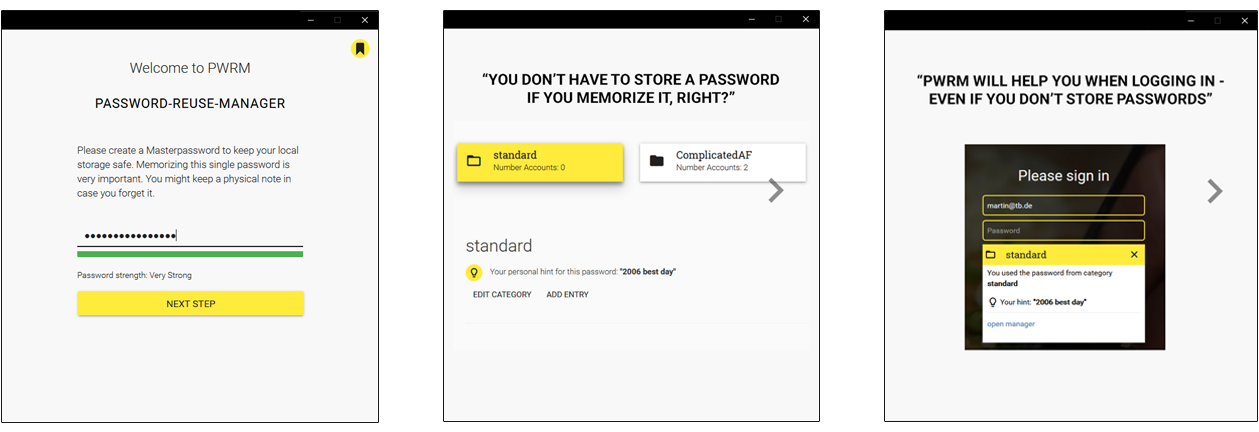
\includegraphics[width=\linewidth]{pwrm/key-screen-2-onboarding}
	\caption{\label{fig:pwrm:key-screen-onboarding} Onboarding wizard.}
\end{figure}

\subsubsection{Extension Home Screen}

\begin{figure}[htbp]
	\centering
	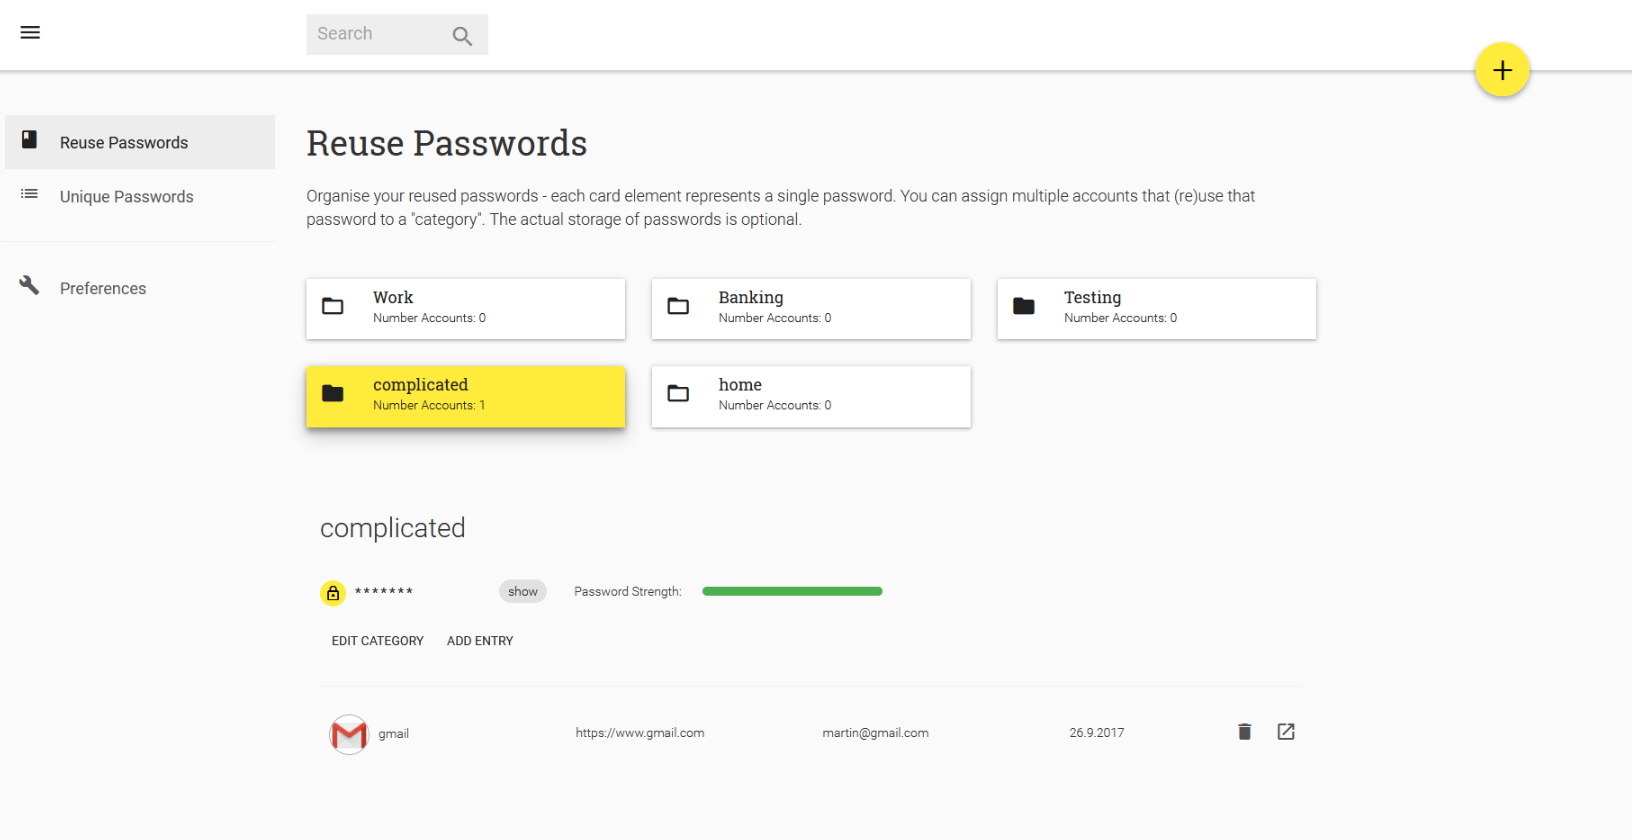
\includegraphics[width=\linewidth]{pwrm/key-screen-1-home}
	\caption{\label{fig:pwrm:key-screen-home} Home screen of the PWRM extension}
\end{figure}

Manual entry of username and password is okay, but not the focus of attention. Kairos 
\begin{figure}[htbp]
	\centering
	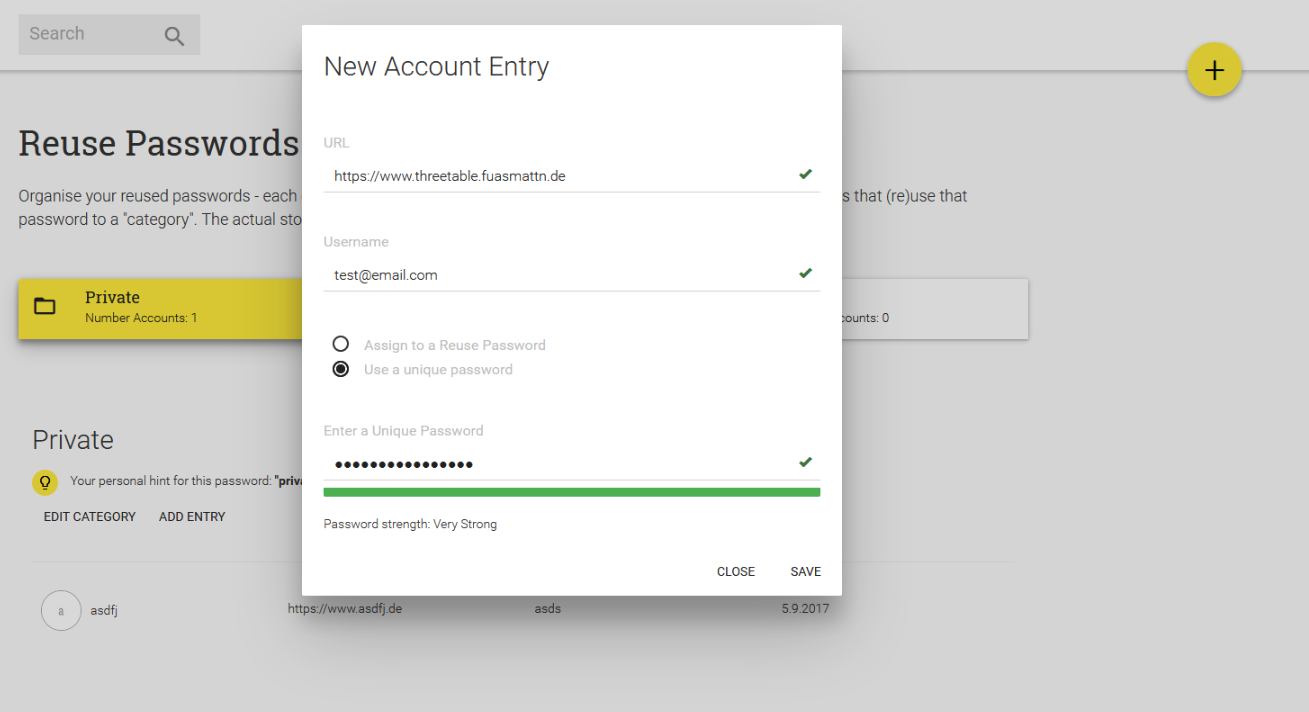
\includegraphics[width=\linewidth]{pwrm/key-screen-3-new-entry}
	\caption{\label{fig:pwrm:key-screen-entry} Manual entry of a new username/password pair. }
\end{figure}

\subsubsection{Interventions}
\begin{figure}[htbp]
	\centering
	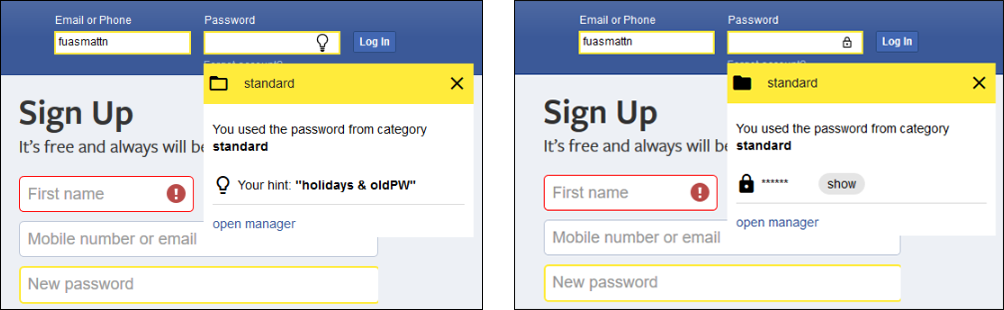
\includegraphics[width=\linewidth]{pwrm/injection-hintboxes}
	\caption{\label{fig:pwrm:injection-hintboxes} }
\end{figure}


\subsection{Implementation}
PWRM is implemented using the WebExtensions API\footurl{https://developer.mozilla.org/en-US/Add-ons/WebExtensions}{05.01.2018}. 
%add some screenshots here
\begin{figure}[htbp]
	\centering
	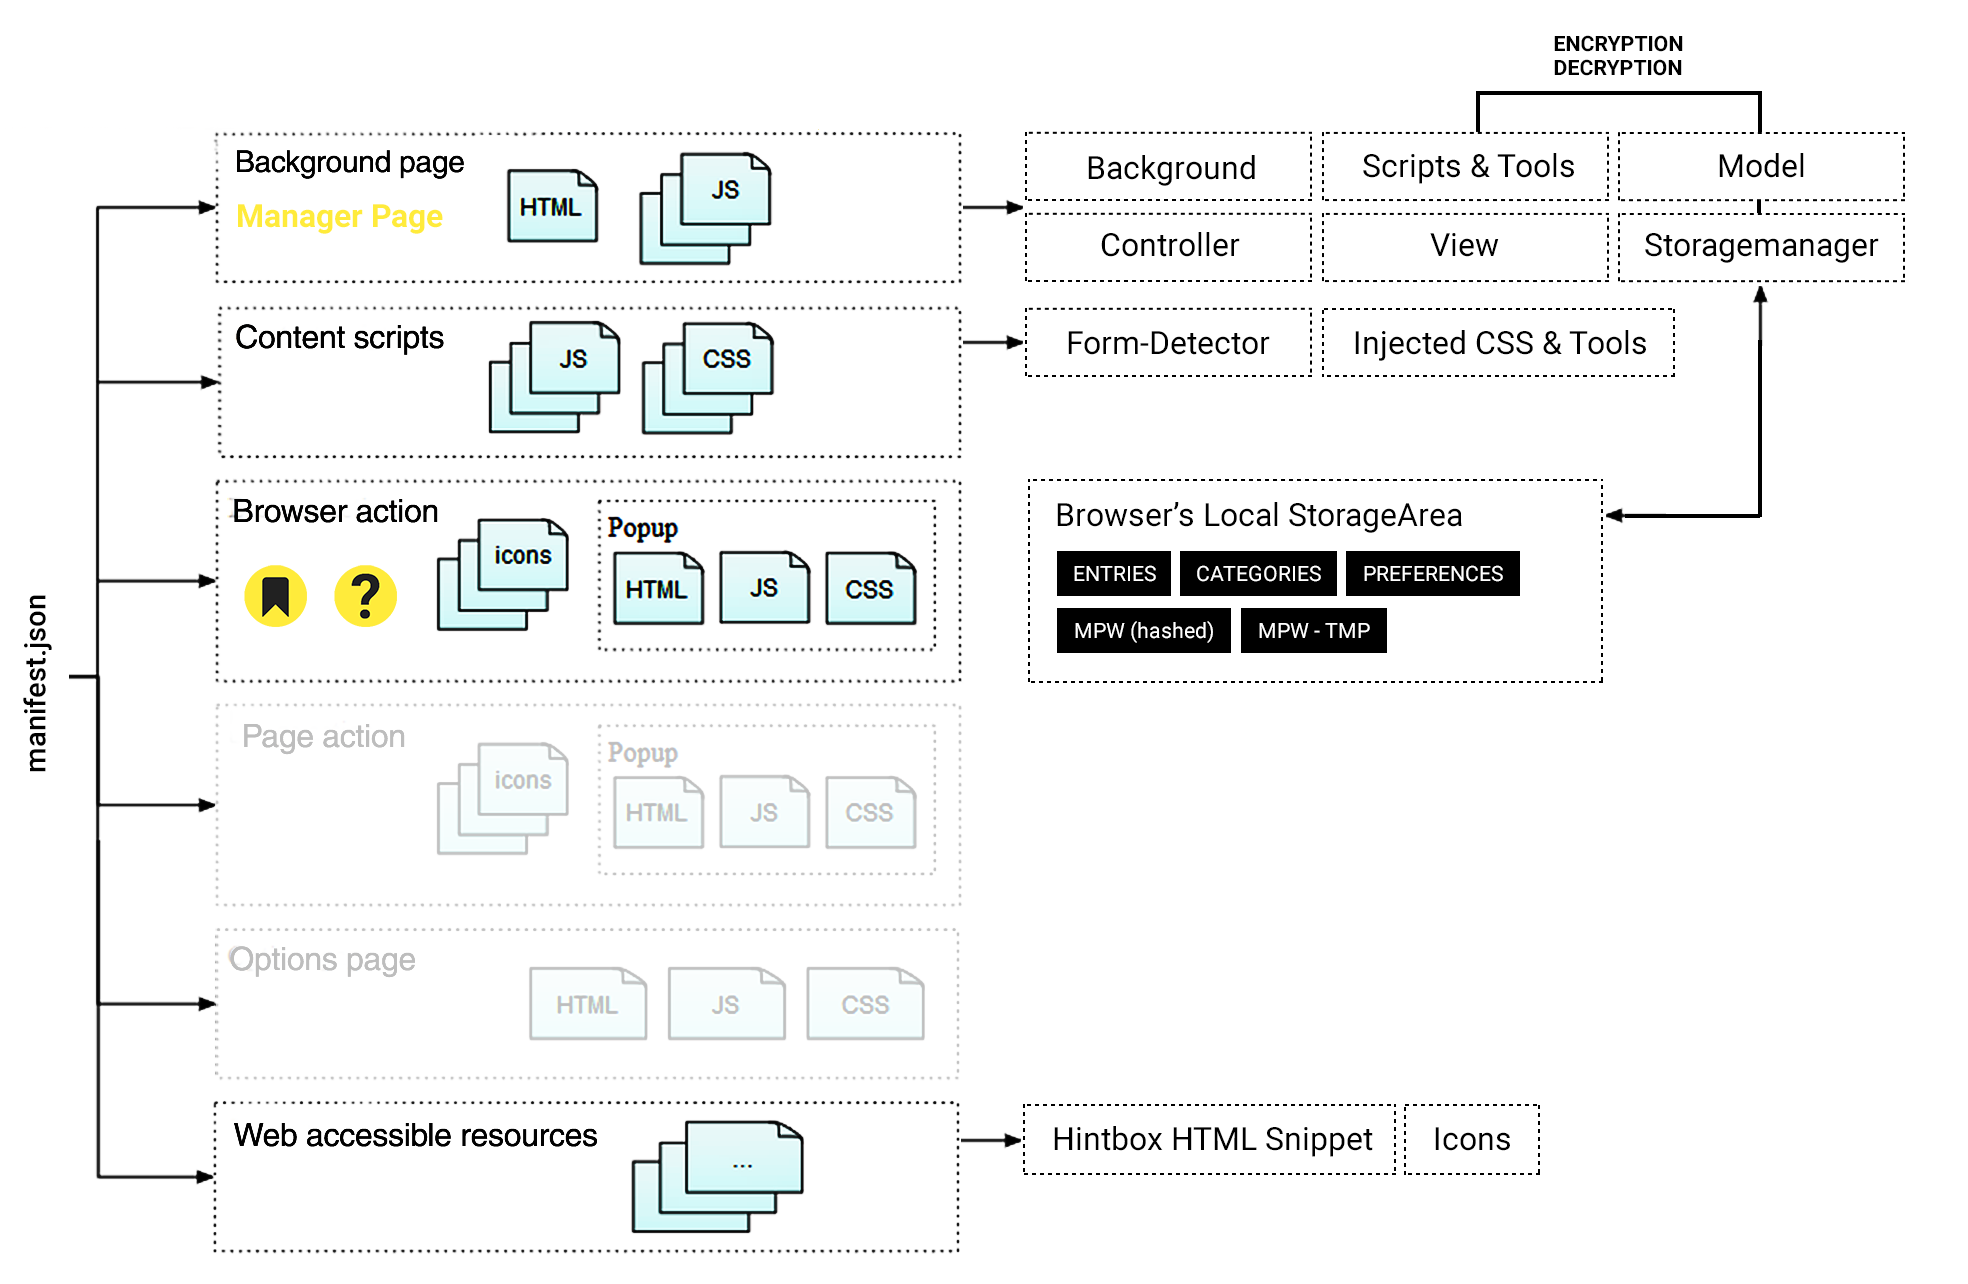
\includegraphics[width=\linewidth]{pwrm/pwrm_anatomy_mod}
	\caption{\label{fig:pwrm:components} Components and Modules of the PWRM WebExtension}
\end{figure}


\section{Field Study}\label{sec:pwrm:field_study}


\subsection{Methodology}



\subsubsection{Recruiting and Demography}
We published the call for participation on social networks


\subsection{Results}

\section{Discussion}
Suggestion of password categories -- can we use the decoy effect here?

\subsection{Limitations}
How well the system works would only be visible in a longer term study. Ten days might not be effective enough to bring out the benefits entirely, but only rough intuitive ratings (which is why we used the INTUI questionnaire)



\section{Lessons Learned and Future Work}

\section{Conclusion}


